\chapter{How Species Separate}

\begin{kaichang}
A zoo poster announces, ``Liger---the offspring of a lion and a tiger!'' Beside it is a photograph of an enormous pale-yellow animal with faint stripes, bigger than either parent.

Wait. Are lions and tigers not different species? School biology says different species cannot produce fertile offspring. Where, then, did this liger come from? Is it a lion, a tiger, or a new species? Turn the question around: your dog and a wolf outside town look very different but can produce healthy pups. Are they one species or two?

Do not look up the answers yet. Write down your guesses. By the end of this chapter, you will discover that ``species'' is much messier than a textbook definition---and that mess is an excellent entrance into evolutionary history.
\end{kaichang}

\section{``Species'' Is Less Clear-Cut Than It Seems}

Begin with observable phenomena.

A horse and donkey can produce a mule, valued by farmers for strength and tolerance of coarse feed. Yet mules almost never become parents: they are sterile. Captive lions and tigers occasionally produce ligers, whose males are also sterile. What about dogs? Chihuahuas and Tibetan mastiffs look like different animals, yet both can produce fertile offspring with gray wolves. Plants offer another contrast: cabbage, cauliflower, broccoli, and Chinese kale are easy to distinguish, but all are cultivars of the same species, Brassica oleracea, and can cross-pollinate and set seed.

Humans deliberately exploit this boundary. Market bananas contain virtually no seeds, and seedless watermelons lack proper seeds. Both are triploid plants whose chromosomes pair chaotically during meiosis, interrupting seed development. The seedlessness farmers desire is essentially artificially created postzygotic isolation.

These contrasts are peculiar: some organisms that ``look like family'' cannot reproduce together, while some that do not resemble each other can. Species boundaries therefore follow neither appearance nor a simple on--off gate. To understand where the line lies, we must zoom into cells and ask what producing offspring requires at the molecular level.

\section{When Chromosomes Prevent Reproduction}

Recall meiosis from Chapter 69: when sperm or eggs form, chromosomes must pair, one paternal set with one maternal set, like two teams joining hands before exchanging segments and distributing them equally. Pairing requires sufficient similarity in chromosome length and gene order, like manuals whose matching page numbers allow comparison page by page.

Consider the mule. Horse body cells have 64 chromosomes, or 32 pairs; donkeys have 62, or 31 pairs. A mule receives 32 from the horse and 31 from the donkey, totaling 63. Trouble arrives when the mule makes reproductive cells: the 32 horse chromosomes and 31 donkey chromosomes differ in number and too much in sequence, leaving many without suitable partners. Disordered pairing disrupts meiosis and prevents normal sperm or eggs. The mule's ``hybrid engine'' runs well enough itself but cannot pass its power onward.

Liger sterility goes a level deeper. Lions and tigers have equal chromosome counts, but millions of years apart have subtly changed their genomes' ``wording habits.'' The same gene turns on at different times and levels in lions and tigers. When both sets occupy one cell, some switching instructions conflict, disrupting reproductive-cell development. Males suffer especially strongly; the challenge section will mention the pattern behind this.

Zoom out slightly, and the particle-level picture of speciation emerges: \textbf{two species are two DNA manuals, once identical, revised until their page numbers no longer match}. How did their revisions diverge?

\section{What Exactly Counts as a Species?}

How much revision makes two species? Biologists still have no single answer. They use several measuring tools, each with applications and limitations:

\begin{table}[htbp]
\centering
\begin{tabular}{p{3.2cm}p{4.6cm}p{4.6cm}}
\toprule
Species concept & Criterion & Clear limitation \\
\midrule
Biological species concept & Can organisms mate naturally and produce fertile offspring? & Cannot handle organisms without mating-based reproduction, such as bacteria and many plants, or fossils \\
Morphological species concept & Are appearance and structure sufficiently similar? & Similarity can be subjective; sexes and life stages within a species may look very different \\
Phylogenetic species concept & Does the group form a distinct branch on an evolutionary tree? & Requires reconstructing the tree first, itself dependent on other evidence \\
\bottomrule
\end{tabular}
\caption{Three common tools for defining species. None works everywhere; biologists choose according to the question.}
\end{table}

School biology's ``reproductive isolation'' uses the first tool, the biological species concept. It works well for most animals and is this chapter's main tool. But remember the last column: it cannot measure bacteria, which lack sexual reproduction, or fossils, whose skeletons cannot be test-mated. Ring species also tie it in knots, as we will see later. More precisely, \textbf{species are a grid humans draw over continuous nature: the grid is useful, but nature has no obligation to fit neatly inside it}.

\section{How Populations Grow Apart}

Having chosen our tool, let us examine speciation in action.

Imagine a mountain valley inhabited by one bird species. A geological event sends a broad river through the valley, separating eastern and western populations that cannot fly across it. This \textbf{geographic isolation} merely starts the timer; it is not yet speciation. The populations then live independently, experiencing Chapter 76's selection and Chapter 77's mutation and drift separately. The dry west favors thick beaks for hard seeds; the wet east favors slender beaks for picking insects. After thousands of years and tens of thousands of generations, beak shape, plumage, and courtship songs differ increasingly.

Eventually the river changes course and the birds meet again. Three outcomes are possible:

\begin{itemize}[itemsep=2pt]
\item They court and mate normally, producing healthy, fertile offspring. Isolation was too short and differences insufficient; they remain one species.
\item They reject one another because songs no longer match or breeding seasons differ, never reaching mating. This is \textbf{prezygotic isolation}.
\item They mate, but embryos stop developing or offspring are sterile like mules. This is \textbf{postzygotic isolation}.
\end{itemize}

The latter two outcomes constitute \textbf{reproductive isolation}. Once stable reproductive isolation develops, the populations truly become two species, no longer sharing genetic changes, like roads extending independently after a fork.

Geographic isolation is the commonest and easiest starting point to understand, but not the only one. Some species separate within one body of water or on one mountain. In a fruit-fly population, for example, individuals preferring to lay eggs on apples and those preferring hawthorns gradually seek mates only on their chosen trees, cutting gene flow themselves. Plants can even form species ``instantly'' through chromosome doubling: triploids are sterile, but doubling to hexaploidy restores normal pairing, immediately isolating the new plant reproductively from its ancestral species. Speciation has many routes; geography is simply the one most often taught.

\begin{table}[htbp]
\centering
\begin{tabular}{p{2.6cm}p{3.4cm}p{6.2cm}}
\toprule
Type & Mechanism & Example \\
\midrule
Prezygotic isolation & Different reproductive times & Two pine species on one mountain shed pollen in February and April, respectively \\
 & Incompatible courtship & Fireflies find mates by flash codes and ignore mismatched signals \\
 & Different microhabitats & One fish species spawns in shallow water and another in deep water in the same lake \\
Postzygotic isolation & Hybrid inviability & Fertilized eggs from two frog species stop developing at the early tadpole stage \\
 & Hybrid sterility & Mules and male ligers \\
\bottomrule
\end{tabular}
\caption{Common reproductive barriers. Prezygotic isolation resembles being unable to arrange a date; postzygotic isolation resembles a partnership breaking down halfway through.}
\end{table}

\begin{qiaoliang}
There is no starting gun for speciation; differences accumulate gradually. How fast? Chapter 77 said each newborn carries about 70 mutations absent from both parents: roughly $6\times10^{9}$ bases in the diploid genome times a per-site, per-generation rate of about $1.2\times10^{-8}$. If two populations are completely isolated with 20-year generations, each undergoes about 50,000 generations in a million years, accumulating roughly $70\times 50000=350$ ten-thousand new differing sites, or 3.5 million, from mutation alone. This excludes selection's amplification of some differences' frequencies. Thus \textbf{even without any ``effort,'' time continually rewrites both manuals}. Once geographic isolation lasts on the million-year scale, reproductive isolation becomes highly probable. Conversely, continual interbreeding by a few migrants dilutes differences through gene flow, delaying speciation.
\end{qiaoliang}

\section{Drawing History as a Tree}

Once species separate, they do not merge again, with very few animal exceptions. Speciation history therefore naturally forms an ever-branching tree: an ancestral species divides, then each branch subdivides. Drawing these relationships produces a \textbf{phylogenetic tree}, this chapter's main symbolic representation and its most easily misread figure.

The tree below shows relationships between humans and several living primates. It depicts their order of separation, not their appearance:

\begin{center}
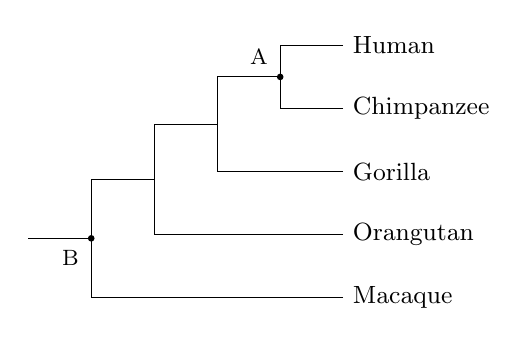
\begin{tikzpicture}[font=\small]
\draw (5.0,4.0) node[right]{Human} -- (4.2,4.0);
\draw (5.0,3.2) node[right]{Chimpanzee} -- (4.2,3.2);
\draw (4.2,3.2) -- (4.2,4.0);
\draw (5.0,2.4) node[right]{Gorilla} -- (3.4,2.4);
\draw (3.4,2.4) -- (3.4,3.6);
\draw (3.4,3.6) -- (4.2,3.6);
\draw (5.0,1.6) node[right]{Orangutan} -- (2.6,1.6);
\draw (2.6,1.6) -- (2.6,3.0);
\draw (2.6,3.0) -- (3.4,3.0);
\draw (5.0,0.8) node[right]{Macaque} -- (1.8,0.8);
\draw (1.8,0.8) -- (1.8,2.3);
\draw (1.8,2.3) -- (2.6,2.3);
\draw (1.0,1.55) -- (1.8,1.55);
\fill (4.2,3.6) circle (1.2pt) node[above left=1pt]{\footnotesize A};
\fill (1.8,1.55) circle (1.2pt) node[below left=1pt]{\footnotesize B};
\end{tikzpicture}
\end{center}

Three rules suffice to read it:

\begin{itemize}[itemsep=2pt]
\item \textbf{Branch points are common ancestors.} Node A represents humans' and chimpanzees' most recent common ancestor, an ancient ape population living roughly six or seven million years ago. It was neither human nor a modern chimpanzee but their shared ``grandmother's grandmother's grandmother'' far back in time.
\item \textbf{Branches can rotate freely around nodes.} Put chimpanzees above humans, or humans at the far left, and the tree means exactly the same thing. Tip order reflects the illustrator's layout, not any degree of advancement.
\item \textbf{All tips are ``contemporaries.''} Every terminal species is alive today, and all have existed on Earth for equally long lineages reaching back to a common ancestor 3.8 billion years ago. A macaque is not a ``monkey stuck halfway.'' It is a relative that separated from us earlier and has evolved along its own path for over thirty million years.
\end{itemize}

\begin{wuqu}
``Evolution is a ladder from lower to higher: bacteria are most primitive, humans most advanced, and today's monkeys will eventually become humans.'' This is the deepest misreading of phylogenetic trees. First, a tree is not a ladder. Ladders have a direction and a top; each evolutionary fork simply sends populations toward their own environmental adaptations, with neither climbing toward the other. Bacteria have lived on Earth for 3.8 billion years and remain the most abundant and widespread life; by successful-living standards, they lose to no one. Second, humans did not descend from today's monkeys. Humans and chimpanzees are cousins, not grandparent and grandchild, sharing node A's ancestor before following separate paths. Asking why monkeys have not become humans is like asking why your cousin has not become you: your cousin has a separate genealogy and life, never a route toward becoming you. Replacing the ladder in your mind with an endlessly branching, topless bush is this chapter's most important mental move.
\end{wuqu}

This representation can extend to the deepest level. Combine sequence and structural evidence from all living organisms, and they connect into one great tree: bacteria, archaea, and eukaryotes including you form three main branches. At the root stands life's last universal common ancestor, an ancient cell population from about 3.8 billion years ago. You, the pothos on your windowsill, and E. coli in a dish all connect through its branch points. This is no mere metaphor: your cells' protein-making ribosomes and basic DNA-reading code use the same parts and language (Chapter 71), compelling evidence of homology. Viruses lack their own ribosomes, and whether they count as full members of this tree remains debated; Chapter 79 returns to that question.

Why trust the tree? Why believe whale ancestors once walked on land? The next section explains how scientists know.

\begin{zhengju}
Nineteenth-century observers saw whales as ``big fish.'' In \emph{On the Origin of Species}, Darwin dared suggest that bears feeding in water could evolve into whale-like creatures, earning prolonged newspaper mockery. Nobody expected three independent evidence streams to converge more than a century later.

The first came from \textbf{fossils}. Beginning in 1979, paleontologists excavated a sequence of roughly fifty-million-year-old animals from ancient Pakistani riverbeds. Pakicetus had characteristic whale ear bones but walking limbs. Slightly later Ambulocetus had strong limbs for supporting its body on land and paddling. Later still, Basilosaurus was a fully aquatic giant retaining absurdly small hind legs: complete bones and joints, but no hope of reaching the ground. Arrange the fossils chronologically, and limb bones shrink step by step while nostrils migrate toward the skull's top.

The second came from \textbf{comparative anatomy and embryos}. Modern whale flippers contain bones arranged remarkably like your arm's: one upper-arm bone, two forearm bones, wrist bones, and five finger bones, with the fingers enclosed in the flipper. Better still, early whale embryos develop hindlimb buds that subsequently stop growing, briefly opening and then closing an obsolete ``ancestral blueprint.''

The third came from \textbf{molecular sequences}. In the 1990s, comparisons of whale and other mammalian DNA surprised everyone: the closest living sequence match was no fishlike creature but the hippopotamus. Researchers subsequently found shared genomic ``scars,'' virus-derived sequences inserted at matching positions, and fossil candidates for their common ancestors, ancient even-toed ungulates called anthracotheres. Whales were even reclassified within Artiodactyla: taxonomically, they are ``hippo relatives that went to sea.''

Three evidence streams from different methods, periods, and laboratories point to the same tree. Science calls this ``convergence of evidence.'' A conclusion supported by independent evidence chains has a much lower chance of being wrong than any one chain alone. Details are still revised, such as the exact placement of early whales. That is science's method: converging evidence stabilizes the broad picture, while new fossils refine the details.
\end{zhengju}

\section{When the Tree Is Less Useful}

A good model recognizes its limits. Nature challenges ``separated populations never merge again'' in several settings:

\begin{itemize}[itemsep=2pt]
\item \textbf{Ring species.} Ensatina salamanders encircle California's Central Valley. Neighboring populations along either side interbreed, passing genes like relay batons, yet the terminal populations meeting at the southern end remain reproductively separate and cannot hybridize. Is this one species or two? Reproductive isolation ties our measuring tool in knots.
\item \textbf{Hybrid zones.} European carrion and hooded crows, black and gray respectively, are clearly two species, yet consistently hybridize where their ranges meet, forming a narrow mixed-color belt that has neither merged nor separated them for tens of thousands of years. On the map, their boundary is a transition zone rather than a line.
\item \textbf{Bacteria do not follow these rules at all.} They lack sexual reproduction and can directly ``hand'' genes to unrelated neighbors through horizontal gene transfer, spreading antibiotic resistance among bacteria. Their genealogy resembles a repeatedly knotted network more than a tidy tree. This is Chapter 79's main subject; here we merely note it.
\end{itemize}

These complications do not make species useless, any more than limits make a map useless. They show that \textbf{speciation is an ongoing continuous process, and labeling arbitrary moments inevitably creates unstable labels}. Ring species are especially valuable: they display the intermediate state of ``one species becoming two'' before our eyes, like a slow-motion replay of speciation.

\begin{tiaozhan}
Why does postzygotic isolation almost always make males sterile first, as with ligers, mules, and fruit-fly hybrids? An empirical pattern called Haldane's rule lies behind this. Geneticists still debate its full explanation, but one mechanism is clear enough to examine. Imagine ancestral genes A and B on one chromosome that must work together. After the population splits, one lineage upgrades A to A', the other B to B'. Each works internally, but when A' and B' meet in a hybrid, the untested combination fails and development stalls. This is Dobzhansky--Muller incompatibility: \textbf{neither mutation is harmful alone; harm comes from independently evolved genes working together for the first time in a hybrid}. Reproductive isolation thus need not involve anyone making a ``mistake''; it can be a byproduct of accumulating divergence. Why are males worse off? They have only one X chromosome, leaving incompatible X-linked genes without a backup to mask them; females have two that can compensate. These details exceed the main thread, and you may skip them without losing what follows.
\end{tiaozhan}

\begin{shiyan}
\textbf{Observation: Two Similar Animals Live Differently}

Materials: notebook and pen; optional binoculars or a phone camera.

Procedure:
\begin{enumerate}[itemsep=1pt]
\item Choose two common, easily confused birds in a neighborhood or park, such as sparrows and light-vented bulbuls, or two similar insects, such as small cabbage whites and Indian cabbage whites.
\item Observe for one week, morning and evening, for 15 minutes each time. Record their positions---ground, shrubs, or treetops---food, most active times, and differences in calls or flight.
\item At week's end, make a comparison table. Did they court one another or compete for the same food? Along which dimensions did their lives differ?
\end{enumerate}

What to observe: match each difference to the isolation-mechanism table. Which categories contain differences in timing, space, and behavior?

Safety reminder: observe only. Do not catch or feed animals or approach nests. Tell a parent about outdoor activities and go with a companion.
\end{shiyan}

\section{Back to the Zoo Poster}

We can now answer the opening questions.

The liger's existence actually confirms that lions and tigers \textbf{are already separate species}, rather than refuting the concept. Three reasons support this. First, wild lions inhabit African savannas and Indian woodlands, while tigers inhabit Asian forests, so their ranges never meet; ligers result only from artificial captive pairings. Second, even when paired, postzygotic isolation appears immediately: all male ligers are sterile, showing that the genomes no longer cooperate properly. Third, the lineages have evolved separately for millions of years and differ greatly in form, hunting, and social behavior. A liger is no ``new species'' but an awkward display of residual relatedness, like two manuals with mismatched page numbers that can still barely cross-reference a few passages.

Dogs and wolves illustrate the opposite. Dogs were domesticated from wolves a little over ten thousand years ago, leaving too little time for their manuals to diverge far, so they can still exchange information. Biologists even classify dogs as a gray-wolf subspecies rather than a separate species. Extreme appearances, such as Chihuahuas versus Tibetan mastiffs, dramatize artificial selection's rapid rewriting of a few developmental-switch genes. Chapter 79 will show how tiny regulatory changes can create large morphological waves.

This tree-not-ladder perspective extends far beyond zoos:

\begin{itemize}[itemsep=2pt]
\item \textbf{Tracing infectious disease.} During COVID-19, scientists drew phylogenetic trees from viral sequences worldwide to see where variants entered and spread. Trees became epidemiologists' maps.
\item \textbf{Protecting biodiversity.} With limited conservation funds, which species should come first? Trees identify species representing entire ancient lineages alone, such as the platypus; protecting them preserves a larger stretch of evolutionary history.
\item \textbf{Crop breeding.} Wild crop relatives are important gene stores. Knowing which relatives are close enough to cross tells breeders which hillsides may supply drought- or disease-resistance genes.
\end{itemize}

Yet our tree makes a tacit assumption: genes travel vertically, from parents to offspring, generation after generation. Bacterial gene exchange hints that life's history has breached this assumption repeatedly. Genomes duplicate themselves, borrow fragments, and refit old components into new machinery. These nonvertical stories belong to the next chapter.

\section*{Try It Yourself}

\begin{sikaoti}
\item Draw a phylogenetic tree containing humans, chimpanzees, and macaques, marking the human--chimpanzee most recent common ancestor. Redraw it after rotating the node leading to chimpanzees and explain why both drawings represent the same relationships.
\item A frog occurs on both sides of a large river. Western populations spawn in spring and eastern ones in summer. What reproductive barrier is this? If an upstream dam makes water temperatures similar and spawning times gradually overlap, how might the populations' evolutionary futures change? Explain.
\item Mules are sterile because their 63 chromosomes cannot pair normally in meiosis. Suppose hybrids between two related plant species are fully fertile. From this information alone, what might you infer about their chromosomes and time since divergence?
\item In a ring species, A can mate with B and B with C, but A cannot mate with C. How many species are A, B, and C under the biological species concept? State in one sentence the difficulty this exposes in defining reproductive isolation.
\item A classmate says, ``Humans are the most advanced animals because they sit at the evolutionary tree's top.'' Draw your understanding of the tree's shape and rebut the statement using each of the three reading rules.
\item Suppose two completely isolated populations each accumulate 70 new mutations per generation, with 25-year generations. Estimate the combined number of different mutated genome sites after two million years of divergence. What factors that could increase or decrease real differences does this estimate ignore?
\end{sikaoti}
